\section{深層類神經網路}

\subsection{簡介}

  深層類神經網路(Deep Neural Network,DNN)又稱「人工類神經網路(Artificial Neural Network,ANN)」,是由神經科學中連結主義(Connectionism)學派的麥氏(McCulloch)與皮氏(Mitts)等人,在 1943 年 \cite{mcculloch_logical_1943} 提出的計算模型。該學派主張藉由模仿生物神經連結的方式建立模型,以建立系統模擬各種心智現象,而其中深層類神經網路由於它在貼合目標函數上的彈性和運算上易於平行化的特徵,得以恰當利用圖形處理器(Graphics Processing Unit,GPU)等硬體裝置的優勢,能夠很好的結合最佳化演算法對貼合(Fit)資料分佈、找出最好的函數(Function),在各類任務與應用上取得前所未有的效能,因而近年為機器學習與電腦科學領域獲得重大進展,現已成為人工智慧發展的主流。

  深層類神經網路最基本的單位是「神經元(Neuron)」,其本質為一個線性分類器,為了模擬生物神經細胞接收訊號、處理到傳出的過程。每個神經元會接收一串數字 \((x_1, x_2, \cdots\cdots, x_N)\) 作為輸入後,得出一個數字 \(y\) 作為輸出。其關係可用下列數學運算式描述:
$$y=\sigma(w^\top x + b) $$
其中輸入 $x = (x_1, x_2, \cdots\cdots, x_N)$ 被描述為一個 $N$ 維向量,該神經元對每個輸入取值分別給予權重(Weight) $w = (w_1, w_2, \cdots\cdots, w_N)$ 相乘後,再對加權平均的結果加上偏差值 $b$ 當成線性輸出值。最後,為了描述分類器函數的非線性(Non-linear)特性,類似神經細胞觸發與否的過程,此輸出值通常會經過激發函數(Activation Function)$\sigma$ 的轉換後才得到最終輸出值 $y$。常見的激發函數包含線性整流單元(Rectified Linear Unit,ReLU)、S 函數(Sigmoid Function)或雙曲正切函數(Hyperbolic Tangent Function,$\tanh$)等等。


\begin{figure}
    \centering
    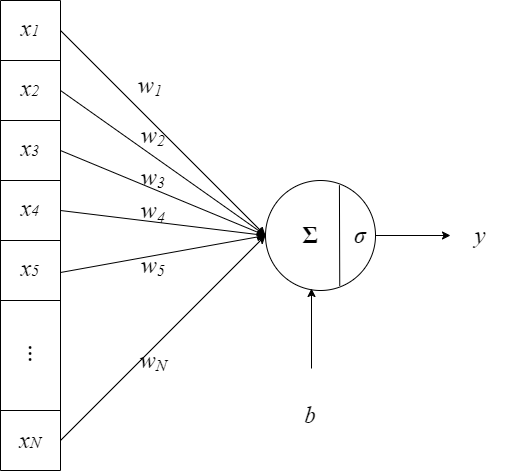
\includegraphics[width=0.5\linewidth]{figures/neuron.drawio.png}
    \caption{神經元示意圖}
    \label{fig:single-neuron}
\end{figure}

  其後羅氏(Rosenblatt)在 1958 年 \cite{rosenblatt_perceptron_1958} 提出感知器(Perceptron),本質上是結合數個神經元的運算,來實現更為複雜的函數功能。基於數學理論中的通用近似定理(Universal Approximation Theorm)\cite{funahashi_approximate_1989},感知器理想上可以近乎模擬一切函數。然而後續研究發現單層感知器具有線性不可分\footnote{例如無法貼合異或(Exclusive OR,XOR)運算等函數}的限制,於是出現了在輸入與輸出函數之間增加隱藏層(Hidden Layer)的多層感知器(Multi-layered Perceptron,MLP),由於在輸入與輸出之間的多層感知器可以藉助隱藏層的幫助實現函數的多次轉換,因而大大拓展了模型的適用範圍。此種計算模型由於是「加深隱藏層」得來的,因而被稱為深層類神經網路(Deep Neural Network)。
  
  然而,單純擁有能夠表達複雜函數的模型是不夠解決現實複雜的工程問題的。為了增加函數貼合的效率,魯氏(Rumelhart)與辛氏(Hinton)等人 \cite{rumelhart_learning_1986, rumelhart_learning_1987} 提出了反向傳播(Backpropagation)演算法,期望藉由計算輸出層與目標函數之間的誤差(Error),透過最佳化演算法計算出梯度(Gradient)後,經由隱藏層反向往輸入層,對整個類神經網路進行修正。於是配合圖形處理器平行運算的能力,資料中貼合函數的過程變得更有效率。如此透過深層類神經網路,找出資料輸入與輸出之間的函數關係的機器學習演算法,就稱之為深層學習(Deep Learning)。由於深層學習的可擴展性(Scalibility)與泛用性(Generalizability),不論在圖像、語音、文字等多個模態,深層類神經網路都已經獲得了廣泛應用,解決更加複雜的現實問題。

  實際上,根據資料特性的不同,並不是所有的資料都能單純的適用於這類輸入與輸出向量直接對應的模式,因此類神經網路又發展出不同的架構以適應資料本身的特性。前述的類神經網路由於運算過程單純是從輸入層經由多層感知器直接進行矩陣運算完成函數的模擬,因此被稱之為「前饋式類神經網路(Feed Forward Network,FFN)」。為了適應各種資料型態的特徵,藉由調整各神經元之間的連接關係,後續發展出了如卷積式(Convolutional)、遞迴式(Recurrent)與轉換器(Transformer)類神經網路等架構,以應對不同任務的需求。由於這些架構在語音與文字處理上相當常用,接下來將一一分別介紹:

\subsection{卷積式類神經網路}

  卷積式類神經網路(Convolutional Neural Network,CNN)為 1998 年由楊氏(LeCun) \cite{lecun_gradient-based_1998} 提出,旨在利用訊號處理上卷積(Convolution)的運算模擬人類視覺皮質感知 \cite{hubel_receptive_1959} 的特性,利用其移動不變性(Shift-invariance)來捕捉二維影像中的局部(Local)特徵,以便後續的類神經網路可以對輸入的資料進行更整體而全面的判斷。

\begin{figure}
    \centering
    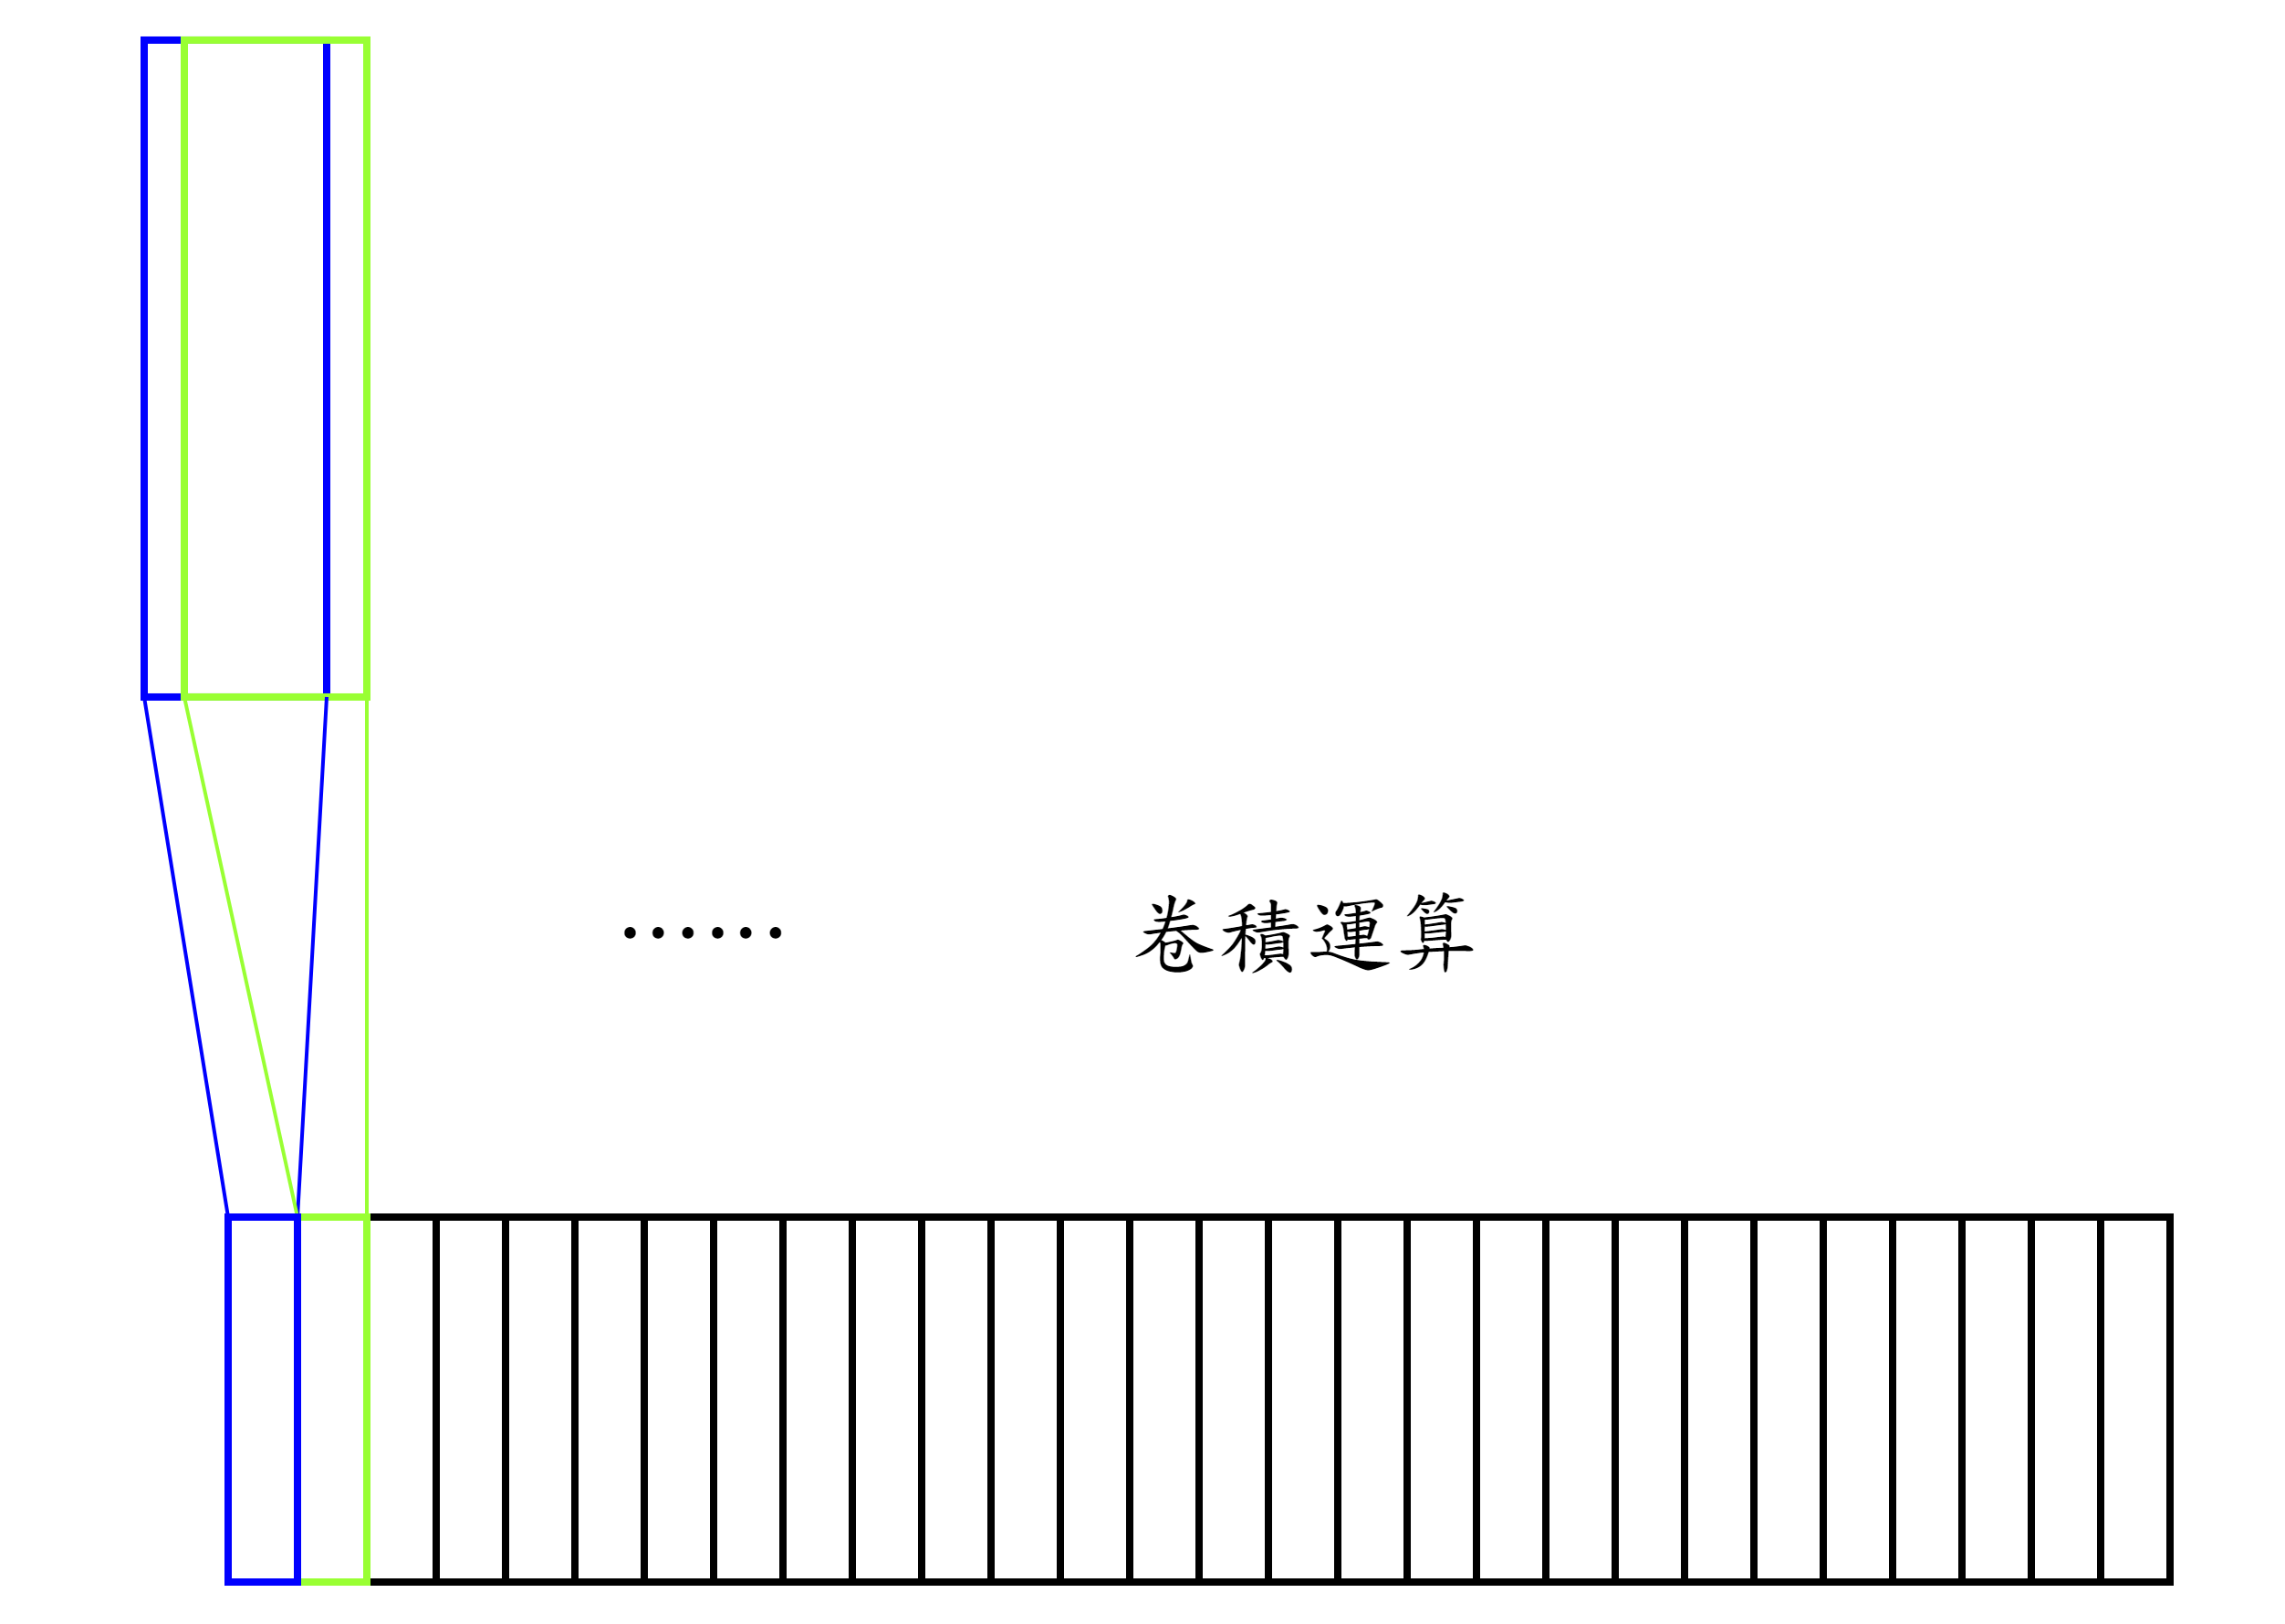
\includegraphics[width=0.5\linewidth]{figures/speechCNN.png}
    \caption{卷積神經網路作用於語音訊號示意圖}
    \label{fig:speech-cnn}
\end{figure}

  有別於圖像中經常是以像素 (Pixel)的三原色亮度進行卷積運算,在語音中卷積式類神經網路的處理對象,除了直接是空氣壓力波形的物理訊號以外,為了更方便機器模型判斷語音訊號的內容,透過聲學知識得到的聲學特徵或深層學習得出的語音表徵,也經常是語音處理中卷積層運算的對象。然而不論是何種輸入,有別於影像的二維資料,語音訊號的資訊是被呈現在時間軸的維度上,因此通常使用一維的卷積式類神經網路,以模仿人耳聽覺對時變訊號的窗框(Window)處理過程,讓模型可以觀察到輸入語音在不同解析度(Resolution)上的資訊,例如本研究特別著重的音位(Phoneme)等。

% // text embedding 先不寫

% // speech acoustic features 拖到後面去寫

\subsection{遞迴式類神經網路}

  不同於運算過程由輸入往輸出單向的前饋式和卷積式類神經網路,為了處理有記憶和狀態的資料,特別是會隨時間變化的序列資訊,在語音和文字的機器學習中,會將輸出訊號重新接回輸入層的遞迴式類神經網路(Recurrent Neural Network,RNN)是一個相當符合語言特性的選擇。此種網路以每個時間點(Timestep)為考慮對象,在每一步會對輸入層的向量進行運算後,不但將此結果算出一個輸出向量,還會得到另外一些數據保留作內部狀態,表示此前經歷過所有序列資料的記憶。常用的 遞迴式類神經網路類型有長短期記憶(Long Short-term Memory,LSTM)和閘門循環單元(Gated Recurrent Unit,GRU),示意圖與運算式分別如下:

%%%%%%%%%%


// 放運算式和示意圖

此類類神經網路通常會以下列介紹的序列至序列的形式被用在如語音辨識、語音合成或機器翻譯等和語言密切相關的任務中。

\subsection{序列至序列(Sequence-to-sequence,Seq2seq)模型}

由於許多以語言為主的資料經常以兩個序列互相配對的形式呈現,因此專門用以處理此類資料的模型被特別稱為序列至序列模型。此類模型一般的架構是由一個編碼器(Encoder)和一個解碼器(Decoder)構成,旨在模擬輸入與輸出序列之間的變化與相依關係(Dependency)。

此類模型一般有兩種模式:

其一是每個時間點都取得一個輸出的向量,用在輸入與輸出等長的任務之中,此模式又被稱為 token classification。

但更常見的狀況是,輸入與輸出兩者序列長度並不總是相同,此時典型的作法是,讓編碼器將輸入序列在每個時間點一一與模型進行運算,藉由內部表徵(Latent representation)的調整對整個輸入序列進行編碼,完成後將最後一個時間點的表徵作為整個序列的代表,此表徵向量會被稱為「語境向量(Context vector)」,接著被傳遞給解碼器依時序生成輸出訊號的序列。

\subsection{專注機制(Attention Mechanism)}

然而由於 RNN 本身需要編碼和解碼的資訊量是整個序列,對時間點距離比較遠的輸入容易被遺忘,也就是難以處理長期相依性(Long-term dependency)的問題。為解決這種困境,Luong 等人提出了「專注機制(Attention mechanism)」,讓解碼器除了依據語境向量的資訊以外,還可以對輸入序列的不同時間點分配權重,在生成輸出序列時重新從輸入序列中得到所需的訊息。

專注機制一般涉及三個向量之間的運算:query、key 和 value,其運算式如下:

(KQV 運算)

具有專注機制的序列至序列模型又被稱為 AED,透過專注機制的引入,大大改善了如語音辨識、機器翻譯等任務的效能。

\subsection{轉換器(Transformer)類神經網路}

儘管 RNN 本身善於處理時序資料,然而它難以平行化的架構限制卻大大束縛了其在訓練和推理(Inference)時的效率。由 attention 獲取靈感,2017 年瓦氏(Vaswani) 等人在 \_\_cite\_\_ 提出了一種完全由專注機制構成,不需依賴遞迴運算的序列至序列模型,用以解決最經典的機器翻譯任務。

\subsubsection{轉換器架構}

轉換器一樣沿用了 Attention 的 KQV 三組向量的邏輯,以 positional encoding 對序列中每個位置的時間點進行編碼,取代原先在 RNN 模型需要一一運算的過程,在實行平行計算的同時也能考慮到資料在不同時間點出現的效應。其整體架構如下:

(tfm 的圖)

(講多頭專注、KQV、FFN 那些)

由於轉換器不需對每個時間點一一運算,使其得以實現高度平行化的優勢,類神經網路得以透過專注機制的幫助同時進行序列資料的大量訓練,這種 scalibility 因而在自然語言和語音處理都獲得了巨大的進展,近乎取代了原先 RNN 的應用場景,近年甚至被電腦視覺的研究者推廣應用在圖像類的資料上( \_\_vit\_\_) ,足以展現此種模型架構的彈性與泛用性,是目前最前沿人工智慧的主流架構。

除了模型架構,機器學習中不可或缺的另一大 component 即是對資料的編碼過程。如何更有效率的讓機器可以理解、處理和輸出,是機器學習乃至深層學習的一大課題。面對捉摸不定、抽象且變化萬千的人類語言,語音和文字處理如何對資料去蕪存菁,表徵學習更是重中之重。

